\chapter{Tools}
\label{chap:tools}
One outcome of the work is a Database and Web application that provide accessibility to biological data, without the need of pre-processing and feature extraction. 
The web server was designed as part of the thesis work and was implemented by two students under the supervision of Dr. Veksler and myself.

This system is intended to resolve the void that relevant data can be mainly found in published papers, and therefore is usually reliant upon authors thoroughness and goodwill. Consequently, there is a lack of data standardization, uniformity and usefulness which lead to difficulties in execution of research studies.

\section{Features}
\begin{enumerate}
\item The system enables the user to retrieve miRNA-target interactions according to specific features such as: miRNA, target gene and several interaction characteristics.
\item The system displays queries results using graphical tools to describe the interactions in addition to raw data. 
\item The system provides a suitable artificial negative data for each positive interaction data for machine learning purposes.
\item The system allows the user to download a formatted file of miRNA-target interactions description.
\item The system provides detailed miRNA-target interactions characteristics, such as: miRNA, target gene, interaction structure, interaction regions, interaction strength, etc.
\end{enumerate}

\section{MirTarFeaturesDB}
Our developed system\\
(\url{http://icc.ise.bgu.ac.il/MirTarFeaturesDB/home})\\
provides a convenient research tool for biologists through a web-based research platform to enable biologists to easily explore, analyze and process biological data. One of the system's main components is a maintainable database which consists of 8 high throughput datasets from a variety of sources. The system supports not only online data retrieval, but also offline data version updates through a dedicated API. This preserves the system's relevance, as it  ensures up-to-date data and also allows future database related adjustments and modifications. Additional important component is an intuitive user interface which would provides unique functionalities, including: miRNA-target interactions retrieval according to specific features, downloading formatted files with detailed interactions characteristics and compatible synthetic negative data, descriptive visual display of results and statistic calculations, etc. These abilities make it easier for researchers to access and use relevant data for comparative exploration purposes, as the system provides a unified data source. They also allow users to generate machine learning models to identify interactions using the supplied artificial negative data.



\begin{figure}[h!]
  \caption{\textbf{Database schema}}
      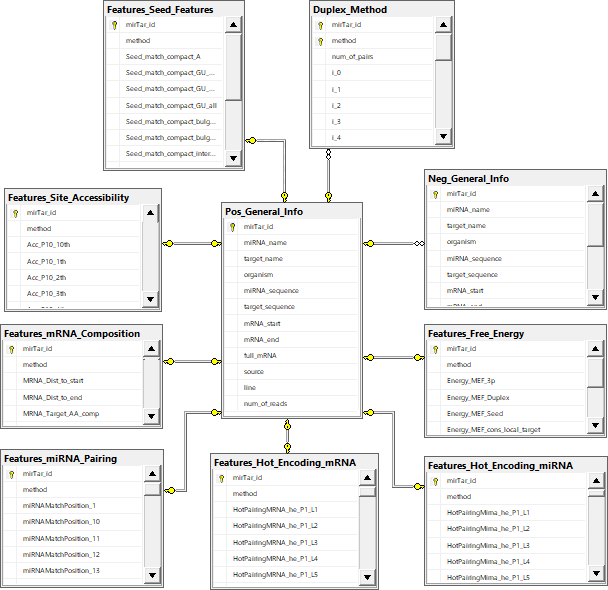
\includegraphics[width = 1\textwidth]{db figures/db schema.png}
      \label{fig:dbschema}
          \end{figure}



\begin{figure}[h!]
  \caption{\textbf{search interaction window}}
      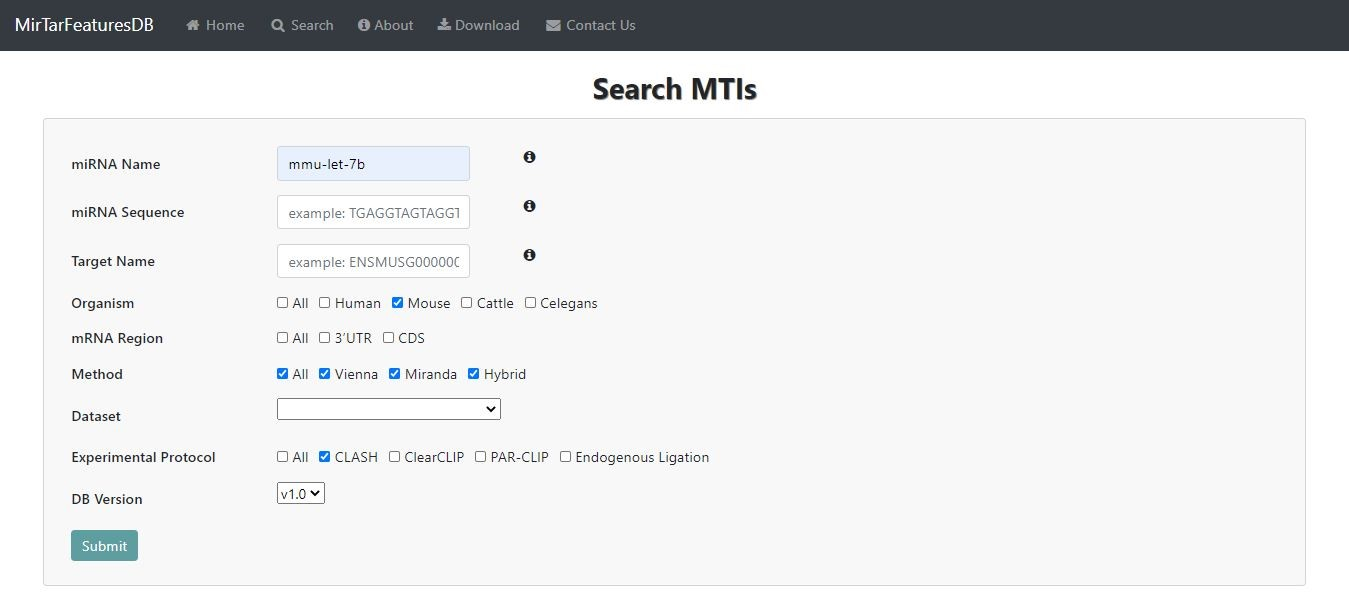
\includegraphics[width = 1\textwidth]{db figures/search interaction window.jpg}
      \label{fig:search}
          \end{figure}



\begin{figure}[h!]
  \caption{\textbf{Result window}}
      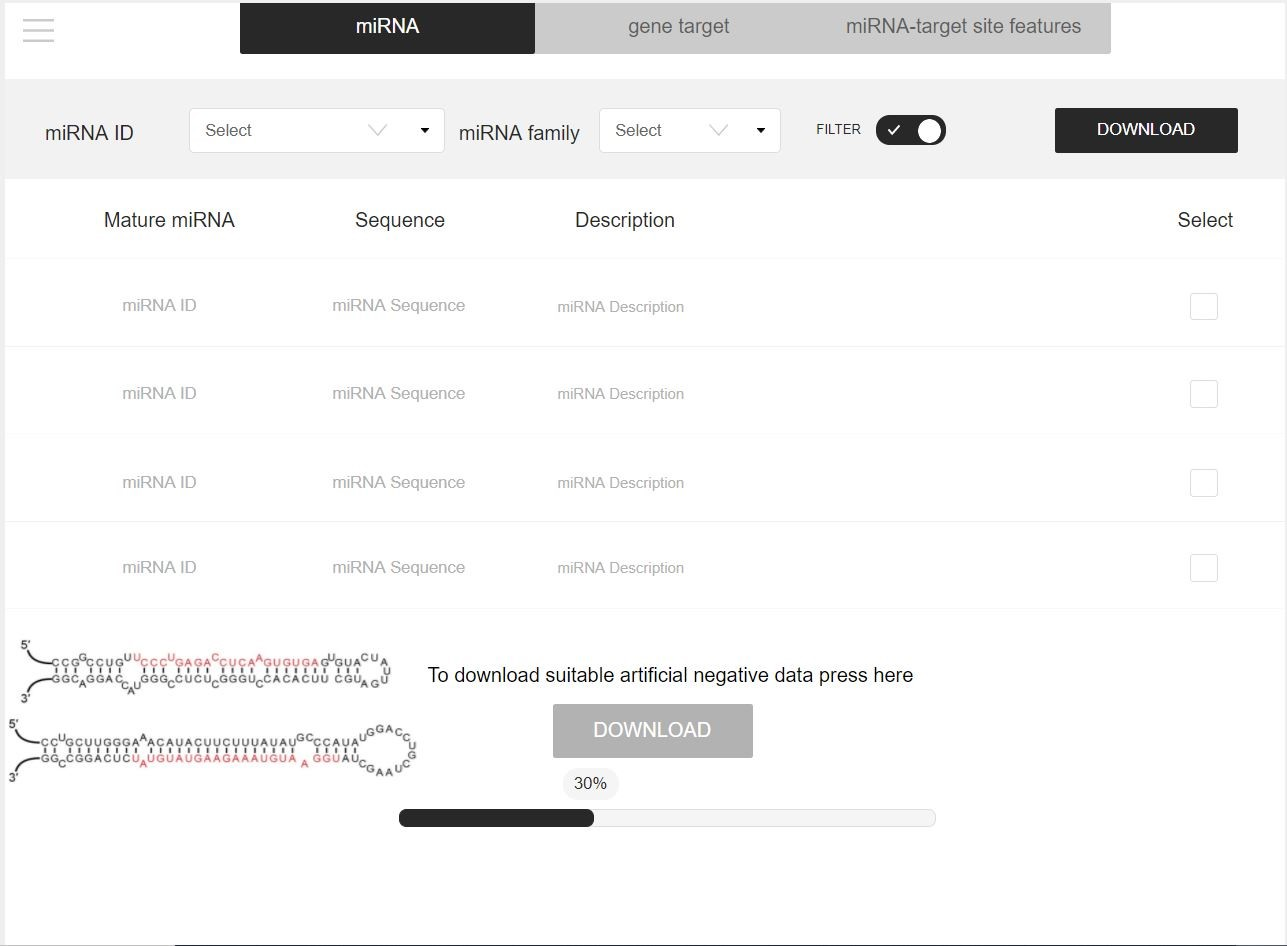
\includegraphics[width = 1\textwidth]{db figures/result.jpg}
      \label{fig:dbresult}
          \end{figure}



\begin{figure}[h!]
  \caption{\textbf{Download interaction file}}
      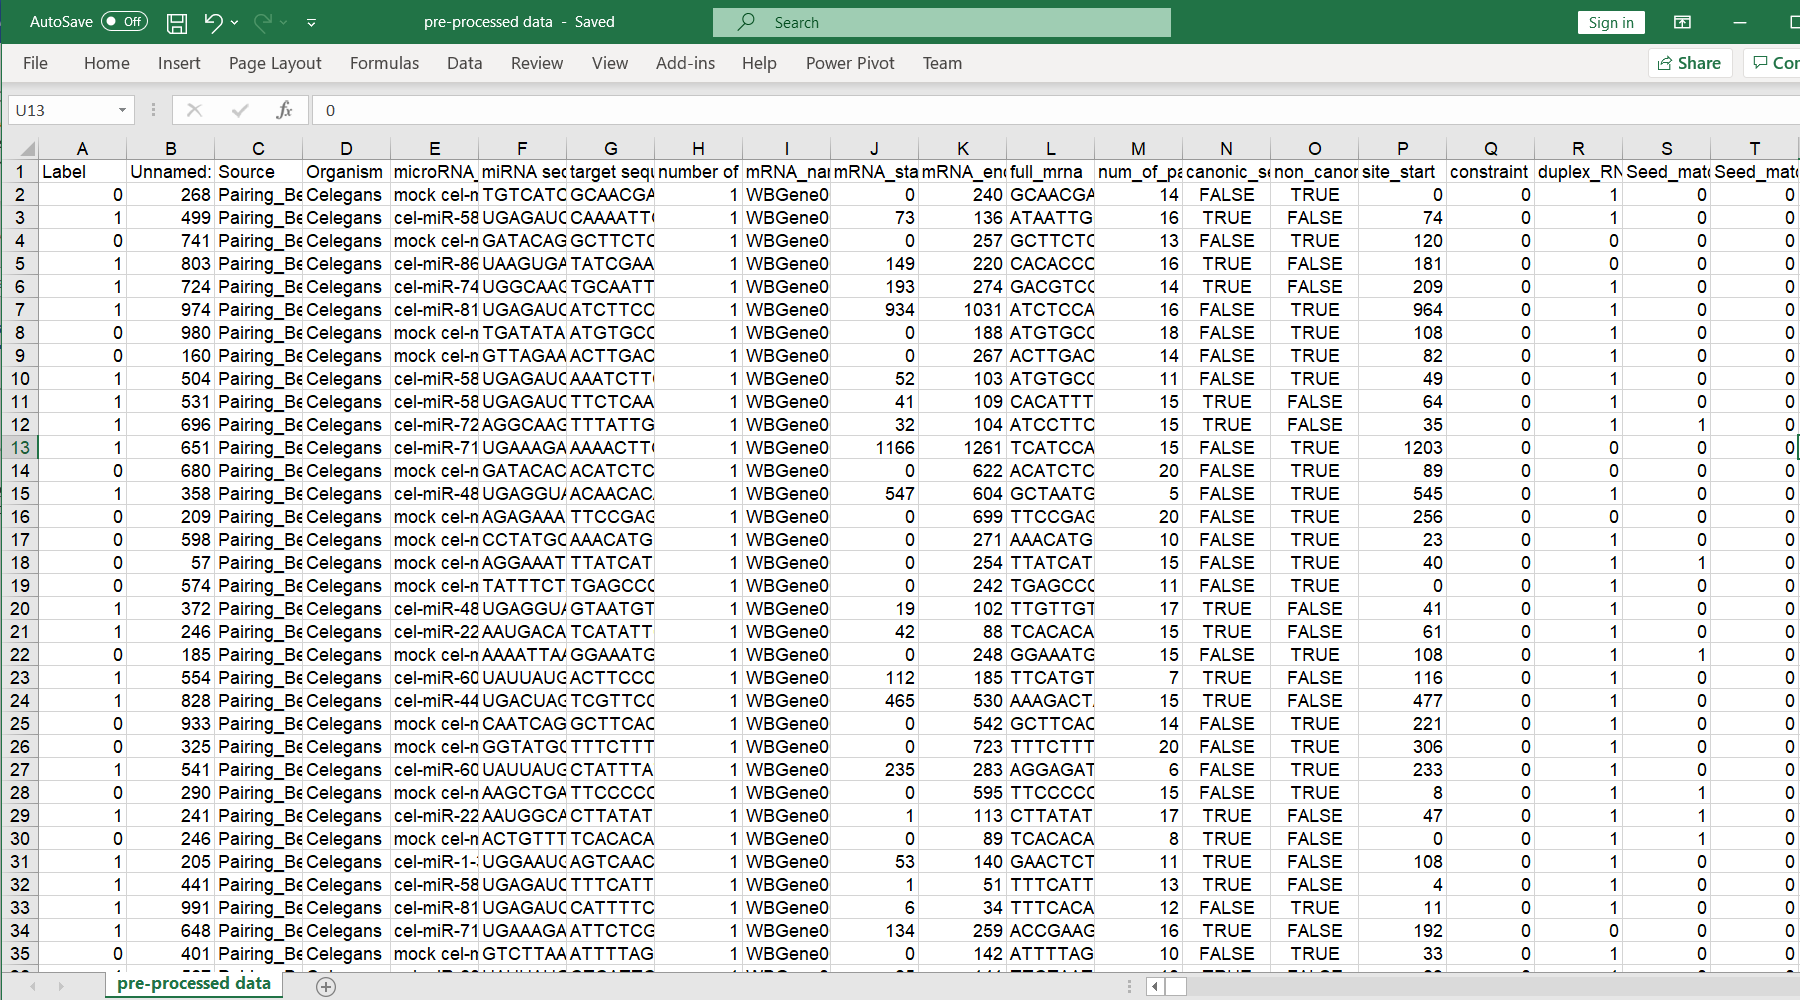
\includegraphics[width = 1\textwidth]{db figures/download.png}
      \label{fig:download}
          \end{figure}

